\documentclass[a4paper]{article}

\usepackage{amsmath}
\usepackage{enumitem}

\usepackage{caption}

\usepackage{subfigure}
\usepackage{amsmath, amssymb}
\usepackage{graphicx}

\DeclareMathOperator*{\argmin}{arg\,min}
\author{Kennard Ng and Luo Wen Han}
\title{Project 2: Latent Dirichlet Allocation}

\bibliographystyle{unsrt}

\begin{document}
	\maketitle
	\section{Introduction}
	
	In this project, we find the underlying population distribution of an individual by its genotype.
	We model this problem using Latent Dirichlet Allocation (LDA) and perform inference on it.
	As inference and learning on LDA is intractable, we use variational inference with mean field assumption to approximate inference in the model. 

	\section{Background}
	
	\subsection{Variational Inference on Latent Dirichlet Distribution}
	\begin{figure}[ht]
		\centering
		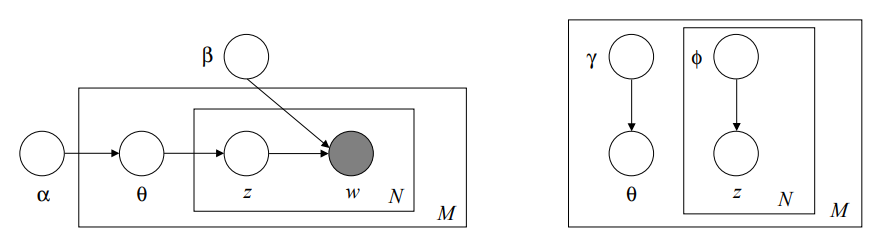
\includegraphics[width=1.0\linewidth]{images/LDA.png}
		\caption{Graphical model representation of LDA (left) and the variational distribution used to approximate the posterior in LDA (right).}
		\label{fig:lda}
	\end{figure}
	Latent Dirichlet Allocation (LDA) is a generative probabilistic model for a collection of discrete data proposed by Blei et al (2003).
	In LDA, documents are represented as random mixtures over latent topics and each topic is represented by a distribution over words.

	LDA assumes the following generative process for each document $w$ in collection $D$:
	\begin{enumerate}
		\item Choose $N\sim Poisson(\xi)$.
		\item Choose $\theta \sim Dir(\alpha)$.
		\item For each of the $N$ words $w_n$:
		\begin{enumerate}
			\item Choose a topic $z_n \sim Multinomial(\theta)$.
			\item Choose a word $w_n$ from $p(w_n|z_n,\beta)$, a Multinomial probaility conditioned on the topic $z_n$.
		\end{enumerate}
	\end{enumerate}

	To perform inference, the posterior distribution of the hidden variables given a document:
	$$p(\theta,z \mid w,\alpha,\beta) = \frac{p(\theta,z,w\mid \alpha,\beta)}{p(w\mid \alpha,\beta)}$$
	must be computed. Unfortunately, computation of this distribution is intractable.
	Instead, approximate inference can be performed on the distribution using variational inference.
	By dropping edges between $\theta, z, w$ and the $w$ node, the following variational distribution is derived:
	$$q(\theta,z \mid \gamma,\phi) = q(\theta\mid\gamma) \prod_{n=1}^{N} q(z_n\mid\phi_n)$$
	where Dirichlet parameter $\gamma$ and the multinomial parameters $(\phi_1,\cdots \phi_N)$ are free variational parameters.
	The graphical representation of both distributions can been seen in Figure \ref{fig:lda}.

	With the simplified distribution, values of the variational parameters $\gamma$ and $\phi$ can be determined
	by minimizing the Kullback-Leibler (KL) divergence between the variational distribution and the true posterior as follows:
	$$(\gamma^*,\phi^*) = \argmin_{(\gamma,\phi)} D(q(\theta,z \mid \gamma, \phi) \parallel p(\theta,z \mid w,\alpha,\beta))$$
	
	By computing the derivatives of the above KL divergence and setting them equal to zero, the following pair of update equations is obtained:
	\begin{align*}
		\phi_{ni} &\propto \beta_{iw_n} \exp{\{E_q[\log{(\theta_i)}  \mid \gamma]\}}, \\
		\gamma_i &= \alpha_i + \textstyle \sum_{n=1}^N \phi_ni.
	\end{align*}
	The expectation in the multinomial update can be computer as follows:
	$$E_q[\log{(\theta_i)}  \mid \gamma] = \Psi(\gamma_i)-\Psi(\textstyle \sum_{j=1}^k \gamma_j),$$
	where $\Psi$ is the first derivative of the $\log\Gamma$ function computable via Taylor approximations.
	
	Since the variational Dirichlet update $\gamma_i$ depends on the variational multinomial $\phi_{ni}$,
	the full variational inference algorithm alternates between the 2 update equations until convergence.

	Note that the variational distribution a conditional distriution conditioned upon $w$,
	as the optimization of the KL divergence is conducted on a fixed $w$.
	\section{Our Approach}
		
	\subsection{Modelling}

	In our problem of classifying individuals in a sample into populations,
	genotype data is measured from each individual.
	We assume the generative process for each genotype data of an individual $w$ in a sample $D$ as follows:
	\begin{enumerate}
		\item Choose $N\sim Poisson(\xi)$.
		\item Choose $\theta \sim Dir(\alpha)$.
		\item For each of the $N$ genes $w_n$:
		\begin{enumerate}
			\item Choose an ancestor population $z_n \sim Multinomial(\theta)$.
			\item Choose a gene $w_n$ from $p(w_n|z_n,\beta)$, a Multinomial probaility conditioned on the ancestor population $z_n$.
		\end{enumerate}
	\end{enumerate}

	We set the number of underlying ancestor populations $K = 4$, and use a previously inferred $\beta$ matrix.
	We can then infer the population mixture $\theta$ and the genotype ancestry assignments $z$ for any individual using variational inference.
	By controlling the value of $\alpha$, we can also control how mixed of ancestor populations each individual has.

	\subsection{Results}
	In our experiment, we performed variational inference on a dataset of 100 indivduals represented by a vocabulary of 200 genotype loci.
	We ran variational inference 4 times with $\alpha = 0.01, 0.1, 1.0, 10.0$.
	\subsection{Iterations and time}
	\begin{figure}[ht]
		\centering
		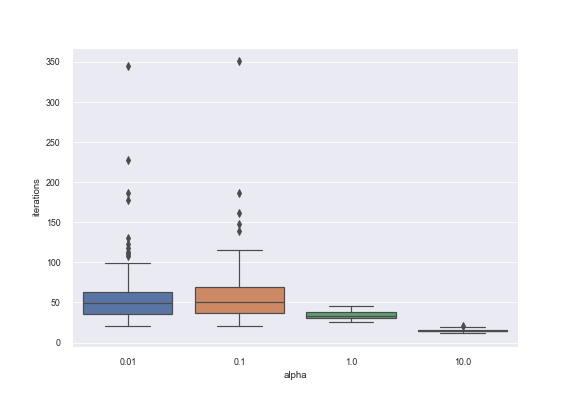
\includegraphics[width=0.8\linewidth]{images/iterations_boxplot.png}
		\caption{Box plot of number of iterations for each $\alpha$ value}
		\label{fig:boxplot}
	\end{figure}
	In figure \ref{fig:boxplot}, we can see the effect of $\alpha$ on the iterations required for convergence.
	The average number of iterations required for convergence is inversely proportionate to the $\alpha$ value specified.
	\begin{table}[ht]
		\centering
		\begin{tabular}{|l|l|}
		\hline
		 & $\alpha$ \\ Time \hline
		 &  \\ \hline
		 &  \\ \hline
		 &  \\ \hline 
		 &  \\ \hline
		 &  \\ \hline
		 \caption{Time of running LDA inference 100 times}
		\label{fig:time}
		\end{tabular}
	\end{table}
	\clearpage
	\bibliography{references.bib}
	
\end{document} 